% source-sha256: 4ffc02b64854cfbbf25954cc04c6e650b5314062bd9d3ba2fcaaaba783a08a57
% Options for packages loaded elsewhere
\PassOptionsToPackage{unicode}{hyperref}
\PassOptionsToPackage{hyphens}{url}
\documentclass[
]{article}
\usepackage{xcolor}
\usepackage[letterpaper,margin=1in]{geometry}
\usepackage{amsmath,amssymb}
\setcounter{secnumdepth}{-\maxdimen} % remove section numbering
\usepackage{iftex}
\ifPDFTeX
  \usepackage[T1]{fontenc}
  \usepackage[utf8]{inputenc}
  \usepackage{textcomp} % provide euro and other symbols
\else % if luatex or xetex
  \usepackage{unicode-math} % this also loads fontspec
  \defaultfontfeatures{Scale=MatchLowercase}
  \defaultfontfeatures[\rmfamily]{Ligatures=TeX,Scale=1}
\fi
\usepackage{lmodern}
\ifPDFTeX\else
  % xetex/luatex font selection
\fi
% Use upquote if available, for straight quotes in verbatim environments
\IfFileExists{upquote.sty}{\usepackage{upquote}}{}
\IfFileExists{microtype.sty}{% use microtype if available
  \usepackage[]{microtype}
  \UseMicrotypeSet[protrusion]{basicmath} % disable protrusion for tt fonts
}{}
\makeatletter
\@ifundefined{KOMAClassName}{% if non-KOMA class
  \IfFileExists{parskip.sty}{%
    \usepackage{parskip}
  }{% else
    \setlength{\parindent}{0pt}
    \setlength{\parskip}{6pt plus 2pt minus 1pt}}
}{% if KOMA class
  \KOMAoptions{parskip=half}}
\makeatother
\usepackage{longtable,booktabs,array}
\usepackage{caption}
\captionsetup[table]{skip=6pt}
\newcounter{none} % for unnumbered tables
\usepackage{calc} % for calculating minipage widths
% Correct order of tables after \paragraph or \subparagraph
\usepackage{etoolbox}
\makeatletter
\patchcmd\longtable{\par}{\if@noskipsec\mbox{}\fi\par}{}{}
\makeatother
% Allow footnotes in longtable head/foot
\IfFileExists{footnotehyper.sty}{\usepackage{footnotehyper}}{\usepackage{footnote}}
\makesavenoteenv{longtable}
\setlength{\emergencystretch}{3em} % prevent overfull lines
\providecommand{\tightlist}{%
  \setlength{\itemsep}{0pt}\setlength{\parskip}{0pt}}
% Release-document layout safeguards injected by scripts/generate_docs.sh.
\usepackage{fvextra}
\fvset{breaklines=true,breakanywhere=true,fontsize=\small}
\RecustomVerbatimEnvironment{verbatim}{Verbatim}{breaklines=true,breakanywhere=true,fontsize=\small}
\setlength{\emergencystretch}{3em}
\AtBeginDocument{\sloppy}
% Workflow-figure support: mermaid blocks in the canonical Markdown are mapped
% to hand-authored TikZ figures by scripts/pandoc_bounded_tables.lua.
\usepackage{tikz}
\usetikzlibrary{shapes.geometric,arrows.meta,positioning,fit,backgrounds,calc}
\definecolor{bdiStep}{HTML}{EAF2FB}
\definecolor{bdiEdge}{HTML}{365F91}
\definecolor{bdiText}{HTML}{17253A}
\definecolor{bdiGate}{HTML}{FFF5D6}
\definecolor{bdiGateEdge}{HTML}{9B6B00}
\definecolor{bdiOpt}{HTML}{F0EAF7}
\definecolor{bdiOptEdge}{HTML}{5B3E86}
\definecolor{bdiOut}{HTML}{E6F4EA}
\definecolor{bdiOutEdge}{HTML}{1E6B3A}
\tikzset{
  bdi/.style={draw=bdiEdge,line width=1pt,fill=bdiStep,text=bdiText,rounded corners=3pt,
              align=center,inner sep=4pt,font=\scriptsize\sffamily},
  bdigate/.style={bdi,draw=bdiGateEdge,fill=bdiGate},
  bdiopt/.style={bdi,draw=bdiOptEdge,fill=bdiOpt,dashed},
  bdiout/.style={bdi,draw=bdiOutEdge,fill=bdiOut},
  bdiflow/.style={-{Stealth[length=2mm]},draw=bdiEdge,line width=0.9pt},
  bdiback/.style={bdiflow,dashed},
  bdilbl/.style={font=\tiny\sffamily,text=bdiText,inner sep=1.5pt,fill=white},
}
\usepackage{bookmark}
\IfFileExists{xurl.sty}{\usepackage{xurl}}{} % add URL line breaks if available
\urlstyle{same}
% fallback for those not using the hyperref driver hyperxmp:
\makeatletter
\@ifundefined{xmpquote}{\newcommand{\xmpquote}[1]{#1}}{}
\makeatother
\hypersetup{
  pdftitle={Business Document Ingestion},
  pdfauthor={Christopher Melhauser and theonlymuffinbot},
  hidelinks,
  pdfcreator={LaTeX via pandoc}}

\title{Business Document Ingestion}
\usepackage{etoolbox}
\makeatletter
\providecommand{\subtitle}[1]{% add subtitle to \maketitle
  \apptocmd{\@title}{\par {\large #1 \par}}{}{}
}
\makeatother
\subtitle{Client Overview}
\author{Christopher Melhauser and theonlymuffinbot}
\date{September 3, 2026}

\begin{document}
\maketitle

\section{Business Document Ingestion: Client
Overview}\label{business-document-ingestion-client-overview}

\subsection{Purpose}\label{purpose}

Business Document Ingestion turns a collection of business records into
a traceable, reviewable data package. It is designed for invoices,
purchase orders, statements, commission reports, receipts, remittances,
shipping documents, credit memos, and related records.

The system does more than read text. It preserves the original evidence,
records how a value was found, checks that values are internally
consistent, and makes uncertainty visible. The goal is to give your team
organized data that can be traced back to the original page before it is
used for reporting, reconciliation, or a later system load.

Courtesy credit is given to Christopher Melhauser and
\texttt{theonlymuffinbot}. \texttt{theonlymuffinbot} describes
collaborative AI tooling and is not a claim of AI legal authorship or
ownership.

\subsection{What the system is designed to
deliver}\label{what-the-system-is-designed-to-deliver}

At the end of a successful run, your team receives a package that can
include:

\begin{itemize}
\tightlist
\item
  preserved source documents and page-level fingerprints;
\item
  extracted fields, line items, tables, and document classifications;
\item
  source citations and raw provider outputs for every AI-assisted
  proposal;
\item
  arithmetic, validation, attribution, completeness, and final-review
  results;
\item
  an Excel workbook, CSV exports, HTML reviewer views, and canonical
  JSON;
\item
  a clear exception list for anything that is missing, ambiguous, or not
  yet authorized; and
\item
  an approved-record staging or retrieval plan when the required gates
  are clear.
\end{itemize}

The system does not silently turn uncertainty into a passing result. A
missing reference, conflicting reading, or unavailable accounting
control remains an explicit exception until it is resolved or formally
retained as an exception.

\subsection{The central rule: evidence
first}\label{the-central-rule-evidence-first}

Every original page and extracted value is retained. A later correction
is an append-only amendment linked to its evidence; it does not
overwrite history. This approach allows a reviewer to answer four
practical questions for any important value:

\begin{enumerate}
\def\labelenumi{\arabic{enumi}.}
\tightlist
\item
  Where did this value come from?
\item
  Which page or source row supports it?
\item
  Which checks did it pass or fail?
\item
  What changed, who authorized it, and when?
\end{enumerate}

AI, mappings, groupings, inferred relationships, and client workbook
imports are proposals until an authorized operator applies an
append-only change and the affected controls are rerun.

\subsection{How the workflow works}\label{how-the-workflow-works}

The process is staged so a later phase cannot erase an earlier failure.

\begin{figure}[htbp]
\centering
\resizebox{\ifdim\width>\textwidth\textwidth\else\width\fi}{!}{%
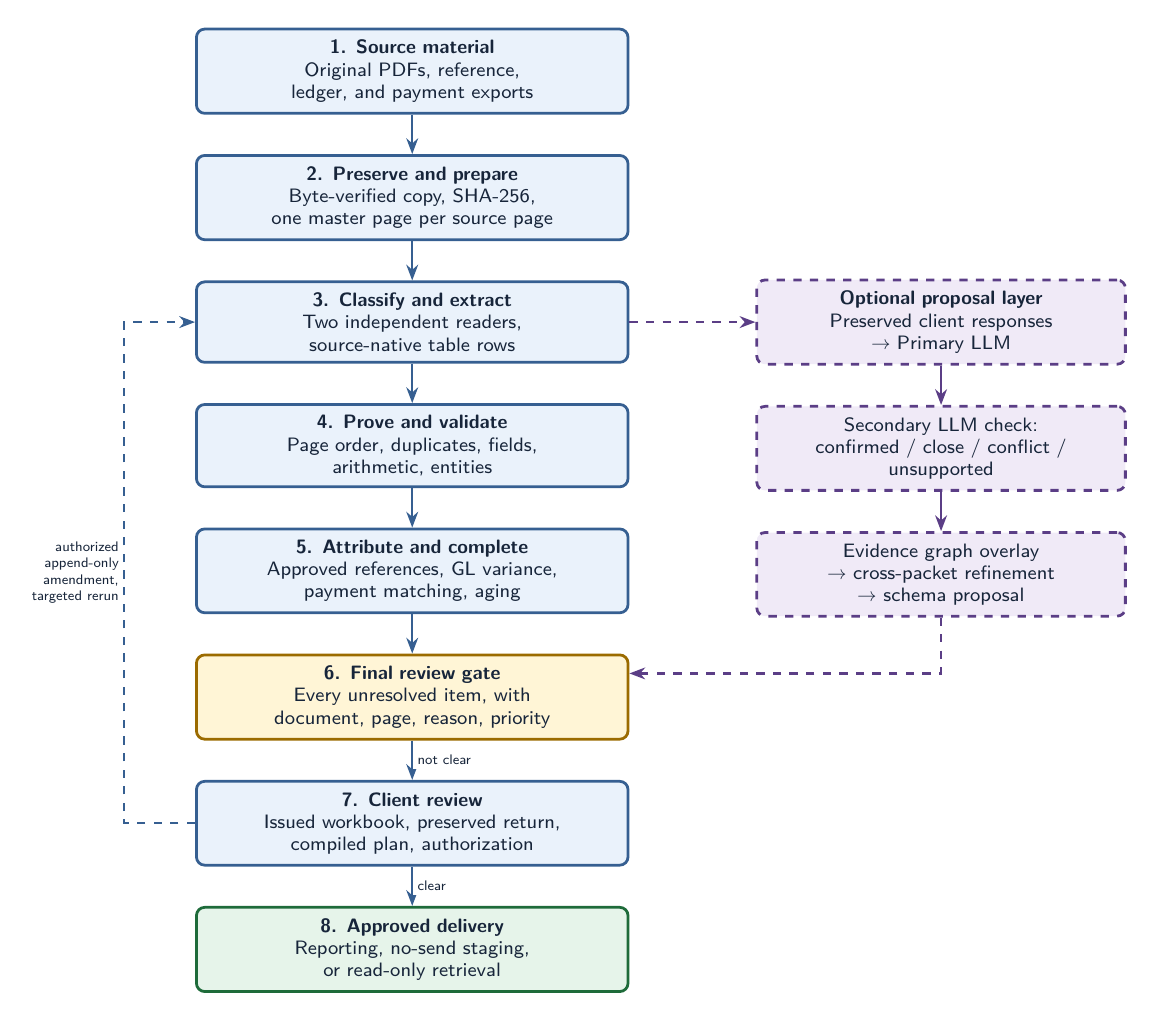
\begin{tikzpicture}[node distance=5mm and 9mm]
  \node[bdi,text width=52mm] (src) {\textbf{1. Source material}\\Original PDFs, reference,\\ledger, and payment exports};
  \node[bdi,text width=52mm,below=of src] (keep) {\textbf{2. Preserve and prepare}\\Byte-verified copy, SHA-256,\\one master page per source page};
  \node[bdi,text width=52mm,below=of keep] (read) {\textbf{3. Classify and extract}\\Two independent readers,\\source-native table rows};
  \node[bdi,text width=52mm,below=of read] (check) {\textbf{4. Prove and validate}\\Page order, duplicates, fields,\\arithmetic, entities};
  \node[bdi,text width=52mm,below=of check] (attr) {\textbf{5. Attribute and complete}\\Approved references, GL variance,\\payment matching, aging};
  \node[bdigate,text width=52mm,below=of attr] (gate) {\textbf{6. Final review gate}\\Every unresolved item, with\\document, page, reason, priority};
  \node[bdi,text width=52mm,below=of gate] (client) {\textbf{7. Client review}\\Issued workbook, preserved return,\\compiled plan, authorization};
  \node[bdiout,text width=52mm,below=of client] (out) {\textbf{8. Approved delivery}\\Reporting, no-send staging,\\or read-only retrieval};

  \draw[bdiflow] (src)--(keep);
  \draw[bdiflow] (keep)--(read);
  \draw[bdiflow] (read)--(check);
  \draw[bdiflow] (check)--(attr);
  \draw[bdiflow] (attr)--(gate);
  \draw[bdiflow] (gate)--node[bdilbl,right]{not clear}(client);
  \draw[bdiflow] (client)--node[bdilbl,right]{clear}(out);

  % Optional proposal layer, to the right of the deterministic spine.
  \node[bdiopt,text width=44mm,right=16mm of read] (llm1) {\textbf{Optional proposal layer}\\Preserved client responses\\$\rightarrow$ Primary LLM};
  \node[bdiopt,text width=44mm,below=of llm1] (llm2) {Secondary LLM check:\\confirmed / close / conflict /\\unsupported};
  \node[bdiopt,text width=44mm,below=of llm2] (llm3) {Evidence graph overlay\\$\rightarrow$ cross-packet refinement\\$\rightarrow$ schema proposal};

  \draw[bdiflow,draw=bdiOptEdge] (llm1)--(llm2);
  \draw[bdiflow,draw=bdiOptEdge] (llm2)--(llm3);
  \draw[bdiback,draw=bdiOptEdge] (read.east)--(llm1.west);
  \draw[bdiback,draw=bdiOptEdge] (llm3.south) |- ($(gate.east)+(0,3mm)$);

  % The authorized-amendment return path.
  \draw[bdiback] (client.west) -- ++(-9mm,0) |- node[bdilbl,pos=0.25,left,align=right]{authorized\\append-only\\amendment,\\targeted rerun} (read.west);
\end{tikzpicture}
}
\caption{Client lifecycle from original evidence to an approved handoff. The deterministic spine (blue) is the only path that can clear a control; the optional proposal layer (purple, dashed) can only add reviewable proposals.}
\end{figure}

The eight stages below match the eight boxes in the diagram above. Each
one states what the stage does, how it does it, and what it produces, so
this section can be read on its own.

\subsubsection{Step 1: The source material you
supply}\label{step-1-the-source-material-you-supply}

\textbf{What it does.} Establishes the evidence base. Everything the
system can later prove is bounded by what arrives at this step.

\textbf{How it does it.} You supply the original source PDFs, unedited,
in the order you received them, together with any available supporting
exports: approved ACK, job, project, PO or order references;
general-ledger data for the matching periods; and payment or remittance
exports. Exports are read with the column headings your system already
prints, so renaming columns is unnecessary and actively harmful --- it
edits the evidence before it is read.

\textbf{What it produces.} The delivery itself becomes retained
evidence. Where an export does not exist, that absence is recorded as a
known limitation rather than being worked around silently.

\subsubsection{Step 2: Preserve and
prepare}\label{step-2-preserve-and-prepare}

\textbf{What it does.} Freezes exactly what was received so that any
later finding can be traced to a specific delivered page.

\textbf{How it does it.} The system keeps the original source, creates a
SHA-256 fingerprint, verifies the retained copy byte-for-byte, and
records a manifest of what was received. PDFs are separated into ordered
one-page masters. For difficult scans, the workflow keeps the grayscale
master and creates enhanced or black-and-white variants beside it; a
profiling pass records contrast, skew, and compression concerns and sets
the handwriting branch.

\textbf{What it produces.} A verified source copy, one immutable master
per page, an intake manifest binding every page to its source file and
position, comparison image variants, and a scan profile. Image
improvements are aids for reading; they never replace the original
source page.

\subsubsection{Step 3: Classify and
extract}\label{step-3-classify-and-extract}

\textbf{What it does.} Determines what each document is and reads the
values printed on it.

\textbf{How it does it.} The system identifies document families and
extracts printed fields, headers, totals, dates, parties, identifiers,
and source-native table rows --- invoice and acknowledgement numbers,
purchase orders, jobs, projects, payment references, commission rates,
customer names, and amounts. Where two genuinely independent extraction
providers are configured, each reads the same page separately and the
readings are compared; the system refuses two lanes that resolve to a
single model vendor, because that is not independent evidence. Tabular
documents are additionally read by a source-native table pass that
follows the layout the document actually uses.

\textbf{What it produces.} Extraction proposals linked to their exact
page, a consensus result recording agreement and disagreement, and
retained raw provider responses. Agreement is useful evidence;
disagreement, a single reading, or a provider failure remains review
work. A provider's confidence score alone is not proof.

\subsubsection{Step 4: Prove and
validate}\label{step-4-prove-and-validate}

\textbf{What it does.} Tests whether the documents hold together
internally, before anything is compared against outside systems.

\textbf{How it does it.} The workflow checks page order and grouping,
surfaces possible duplicates, validates required fields and formats, and
proves arithmetic against source-visible values --- line extensions,
taxes, discounts, freight, credits, subtotals, and document totals. It
resolves entities and addresses through a reversible merge log, and
checks readings for plausibility without inferring a unit, date order,
or country from magnitude.

\textbf{What it produces.} An arithmetic proof result, a validation
result, a reassembly proposal, and a duplicate-candidate list --- each
recording what was checked and what could not be proved. If a number
does not add up, a page sequence cannot be proved, or a handwritten
change conflicts with printed information, the issue stays visible. The
system does not repair it by guessing, and a control that had nothing to
check is reported as failed rather than clear.

\subsubsection{Step 5: Attribute and test
completeness}\label{step-5-attribute-and-test-completeness}

\textbf{What it does.} Connects amounts to your business references,
then measures what the documents alone cannot establish.

\textbf{How it does it.} When your business process requires an amount
to be associated with an ACK, job, project, purchase order, order,
claim, or other reference, the system applies the reference hierarchy
you approve. Where general-ledger and payment or remittance exports are
available, it compares document totals by accounting period, matches
invoices to payments including partial payments, and computes aging.

\textbf{What it produces.} An attribution result with a full evidence
chain per amount; an unattributable register listing every amount that
could not be linked, with its reason and value; and a completeness
report with period variances, payment matches, and aging status.
Unmatched rows are reported back with their original heading and content
rather than dropped. Unmatched amounts are never assigned to a
convenient but unsupported reference, and a variance is reported rather
than plugged.

Authoritative ledger and payment records are categorically different
from document evidence, and are required to close the corresponding
controls. Where they are absent, see the inferred-proposal section
below.

\subsubsection{Step 6: The final review
gate}\label{step-6-the-final-review-gate}

\textbf{What it does.} Collects everything unresolved into one queue and
decides whether the run may advance.

\textbf{How it does it.} Every review-bearing artifact from every
preceding stage --- including recovery artifacts --- is gathered into a
single exhaustive queue. Items may be grouped by root cause so one
decision can answer many similar cases, but grouping never removes an
underlying item. Financially material issues are prioritized.

\textbf{What it produces.} The canonical
\texttt{final\_\allowbreak{}client\_\allowbreak{}review.json} queue plus
CSV, Excel, and HTML views of it, and a final reconciliation manifest
stating which controls passed, which were not applicable, and which
remain blocked. This manifest --- not the appearance of the spreadsheet
--- is the authoritative answer to whether the run can advance.

\subsubsection{Step 7: Client review and
authorization}\label{step-7-client-review-and-authorization}

\textbf{What it does.} Captures your decisions without letting any of
them apply themselves.

\textbf{How it does it.} The client-review package identifies the
records that need a decision. When a workbook returns, the issued and
returned copies are preserved separately and unchanged. The system
validates the workbook structure against the issued copy, records every
response and note into a preserved-response snapshot, and verifies that
no response was omitted or altered. An operator then compiles a change
plan stating exactly which mapping, amendment, or policy change is
affected, which documents and fields are involved, and which downstream
controls must rerun. Each proposed change is authorized individually,
bound to the unchanged plan; anything not chosen stays deferred rather
than being treated as a silent no.

\textbf{What it produces.} A preserved-response record, a compiled
change plan, an operator authorization bound to that plan, and --- only
then --- applied append-only amendments. This keeps client feedback
visible without allowing a returned workbook to bypass the control
process.

\subsubsection{Step 8: Rerun and approved
delivery}\label{step-8-rerun-and-approved-delivery}

\textbf{What it does.} Re-proves everything downstream of an authorized
change, then produces the handoff.

\textbf{How it does it.} Approved amendments are append-only: the
original value remains in the audit trail beside the amendment. The
affected extraction or mapping lane is rerun, followed by arithmetic,
validation, attribution, completeness, and final review, in that order.
Reruns are written to a new output location so an earlier manifest or
package is never silently replaced.

\textbf{What it produces.} A regenerated package showing both the
original client response and the resulting control status, and --- only
when the gate is clear or the remaining items are explicitly retained as
approved exceptions --- a canonical export, load plan, vendor-neutral
no-send staging package, or read-only retrieval store.

\subsubsection{What each stage produces, at a
glance}\label{what-each-stage-produces-at-a-glance}

{\def\LTcaptype{none} % do not increment counter
\begin{longtable}[]{@{}
  >{\raggedright\arraybackslash}p{(\linewidth - 4\tabcolsep) * \real{0.3333}}
  >{\raggedright\arraybackslash}p{(\linewidth - 4\tabcolsep) * \real{0.3333}}
  >{\raggedright\arraybackslash}p{(\linewidth - 4\tabcolsep) * \real{0.3333}}@{}}
\toprule\noalign{}
\begin{minipage}[b]{\linewidth}\raggedright
Stage
\end{minipage} & \begin{minipage}[b]{\linewidth}\raggedright
Principal outputs
\end{minipage} & \begin{minipage}[b]{\linewidth}\raggedright
Can it clear a control?
\end{minipage} \\
\midrule\noalign{}
\endhead
\bottomrule\noalign{}
\endlastfoot
1. Source material & Retained delivery; recorded gaps & No --- it
defines what is provable \\
2. Preserve and prepare & Verified copy, page masters, intake manifest,
scan profile & No \\
3. Classify and extract & Extraction proposals, consensus result, raw
responses & No --- proposals only \\
4. Prove and validate & Arithmetic proof, validation result, duplicate
and grouping proposals & Yes, for arithmetic and validation \\
5. Attribute and complete & Attribution result, unattributable register,
completeness report & Yes, where authoritative exports exist \\
6. Final review gate & Canonical review queue, reviewer views,
reconciliation manifest & It reports the gate \\
7. Client review & Preserved responses, compiled plan, authorization,
amendments & No --- authorization is not clearance \\
8. Rerun and delivery & Regenerated package, canonical export, staging
or retrieval & Yes, on rerun of the affected controls \\
\end{longtable}
}

\subsection{How the optional AI-assisted relationship process
works}\label{how-the-optional-ai-assisted-relationship-process-works}

The system can use AI to find relationships that deterministic
extraction may have missed. This is useful when no more client data will
arrive and the source documents contain printed ACK, job, project, PO,
invoice, order, payment, remittance, party, or template clues.

The AI process is bounded and evidence-based:

\begin{enumerate}
\def\labelenumi{\arabic{enumi}.}
\tightlist
\item
  The system constructs a packet from retained source records and
  preserved client responses. Client comments are reasoning context, not
  source proof.
\item
  The Primary LLM proposes only source-visible relationships and must
  cite the supporting document and evidence quote.
\item
  An independently configured Secondary LLM checks the same packet and
  labels each proposal \texttt{confirmed},
  \texttt{close\_\allowbreak{}needs\_\allowbreak{}review},
  \texttt{conflict}, or \texttt{unsupported}.
\item
  Confirmed proposals are added as immutable graph overlays; they do not
  change source evidence or canonical data.
\item
  Later passes examine unresolved evidence neighborhoods. The process
  stops when a pass produces no material new, source-backed,
  Secondary-LLM-confirmed relationship or reaches its configured limit.
\item
  A graph-guided cross-packet pass examines related documents that could
  not be matched within a single packet. Its configured neighborhood has
  explicit document and byte limits, with separate exceptions for
  deferred or identifier-less records.
\end{enumerate}

This process can improve reference discovery, relationship modeling, and
understanding of repeated layouts. It cannot create an authoritative
ledger balance, payment-system transaction, or client authorization from
document evidence alone.

\subsection{Schema discovery: how the system learns the
structure}\label{schema-discovery-how-the-system-learns-the-structure}

After retained extraction and relationship evidence are available, the
system can build a proposal-only schema inventory. It identifies
observed field names, counts, examples, document/template families,
repeated line structures, and possible relationships.

The schema-discovery process can propose that a printed label likely
represents a PO, ACK, customer, commission amount, or other business
concept. It does not silently establish that mapping. A high-confidence
proposal still needs clear source-template evidence, independent
Secondary LLM review where configured, and the normal authorization path
before it becomes a reusable rule.

\subsection{What happens when client ledger, payment, or reference
exports are
missing}\label{what-happens-when-client-ledger-payment-or-reference-exports-are-missing}

The system can build clearly labeled inferred-control proposals from
retained document evidence. These may include source-linked attribution
candidates, document-total rollups, explicit printed payment markers,
and a detailed exception register.

These artifacts prioritize work and explain missing evidence. They do
not substitute for a general ledger, payment system, or approved
reference export; the final manifest keeps the corresponding control
blocked unless authoritative evidence or an explicitly accepted
exception is available.

\subsection{The output: what you receive and how to read
it}\label{the-output-what-you-receive-and-how-to-read-it}

The optional development extension can retain original PNG/JPEG page
images and let a connected vision-capable assistant propose
schema-mapped fields. Receipts, unknown labels, uncertainties,
corrections and rejections remain visible. A valid submission means
\textbf{pending review, not published}; it cannot update the approved
database or a CRM. The operator can export a private source archive and,
for complete usable sources, a hash-linked image PDF for normal
profiling/intake. Independent verification, business controls and
authorization still apply. There is no bundled mobile capture app or
attachment relay, and actual upload/vision support needs client
acceptance. Governed record writes and expanded custom analytics remain
development work. The \href{CLIENT_OUTPUT_OVERVIEW.md}{output guide}
explains these capabilities in context;
\href{../references/visual-ingestion.md}{Visual Intake} defines the
technical limits.

This section is the summary of the deliverable. It describes what is in
the package, what each part is for, how to read a result correctly, and
what the package deliberately declines to claim.

For a self-contained explanation of the approved-data package, reports,
MCP/API access, controlled downloads, and CRM-ready inputs, see
\href{CLIENT_OUTPUT_OVERVIEW.md}{\texttt{CLIENT\_\allowbreak{}OUTPUT\_\allowbreak{}OVERVIEW.md}}.
That guide is the plain-language bridge from this delivery package to
safe day-to-day use.

\subsubsection{What is in the package}\label{what-is-in-the-package}

\textbf{1. The canonical review record.}
\texttt{final\_\allowbreak{}client\_\allowbreak{}review.json} is the
complete machine-readable queue and the authoritative list of what needs
a decision. Each item identifies the document and page, the field,
region or relationship in question, the reason it is open, its priority,
and the evidence supporting the proposed reading.

\textbf{2. The reviewer views.}
\texttt{final\_\allowbreak{}client\_\allowbreak{}review.csv},
\texttt{.xlsx}, and \texttt{.html} present that same queue in forms that
are easier to filter, sort, and discuss. They are convenience copies,
not separate records; where they disagree with the JSON, the JSON
governs. The Excel workbook carries \texttt{Header\ Definitions},
\texttt{Schema\ Definitions}, and \texttt{Runbook} sheets so it can be
understood without another file.

\textbf{3. The final reconciliation manifest.} This reports which
controls passed, which were not applicable, and which remain blocked. It
is the authoritative answer to whether the run can advance.

\textbf{4. The evidence and audit trail.} Retained source documents and
page-level fingerprints; extracted fields, line items, tables, and
classifications; source citations and raw provider outputs for every
AI-assisted proposal; the unattributable register and exception
registers; preserved client responses; and every authorized amendment
with its operator and timestamp.

\textbf{5. The onward package, when the gate permits it.} A canonical
export, load plan, vendor-neutral no-send CRM/API staging package, or
citation-backed read-only retrieval store.

\subsubsection{How to read a result
correctly}\label{how-to-read-a-result-correctly}

\begin{figure}[htbp]
\centering
\resizebox{\ifdim\width>\textwidth\textwidth\else\width\fi}{!}{%
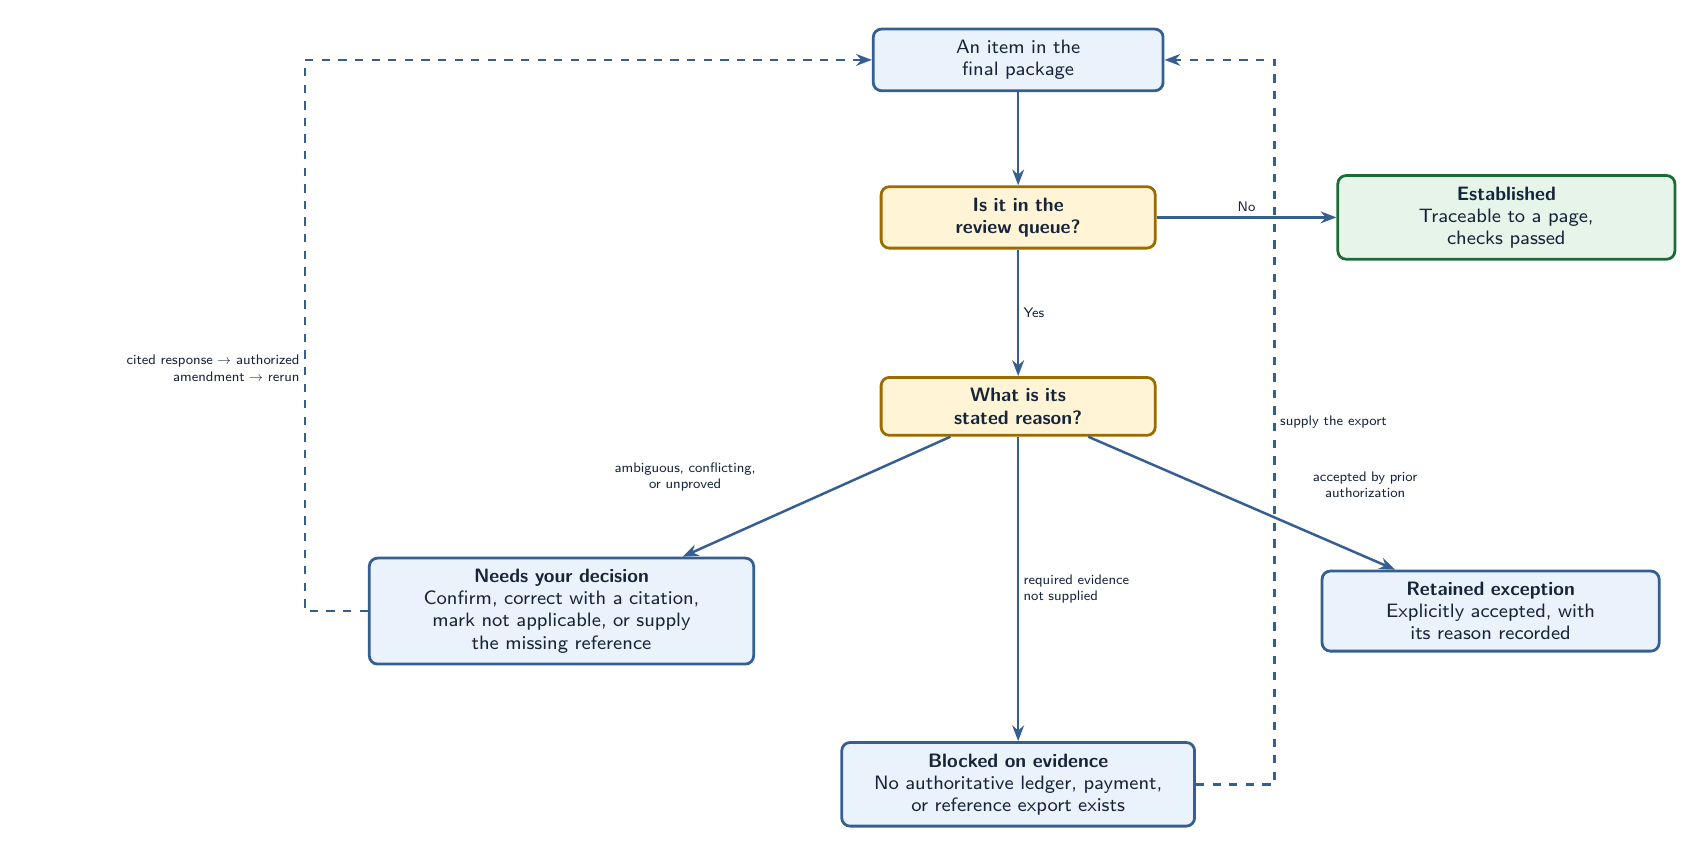
\begin{tikzpicture}[x=1mm,y=1mm]
  \node[bdi,text width=34mm] (I) at (0,0) {An item in the\\final package};
  \node[bdigate,text width=32mm] (Q1) at (0,-20) {\textbf{Is it in the\\review queue?}};
  \node[bdigate,text width=32mm] (Q2) at (0,-44) {\textbf{What is its\\stated reason?}};

  \node[bdiout,text width=40mm] (R1) at (62,-20) {\textbf{Established}\\Traceable to a page,\\checks passed};
  \node[bdi,text width=46mm] (R2) at (-58,-70) {\textbf{Needs your decision}\\Confirm, correct with a citation,\\mark not applicable, or supply\\the missing reference};
  \node[bdi,text width=42mm] (R3) at (0,-92) {\textbf{Blocked on evidence}\\No authoritative ledger, payment,\\or reference export exists};
  \node[bdi,text width=40mm] (R4) at (60,-70) {\textbf{Retained exception}\\Explicitly accepted, with\\its reason recorded};

  \draw[bdiflow] (I)--(Q1);
  \draw[bdiflow] (Q1)--node[bdilbl,above]{No}(R1);
  \draw[bdiflow] (Q1)--node[bdilbl,right]{Yes}(Q2);
  \draw[bdiflow] (Q2)--node[bdilbl,above left,align=center,text width=32mm]
        {ambiguous, conflicting,\\or unproved}(R2);
  \draw[bdiflow] (Q2)--node[bdilbl,right,align=left,text width=30mm]
        {required evidence\\not supplied}(R3);
  \draw[bdiflow] (Q2)--node[bdilbl,above right,align=center,text width=30mm]
        {accepted by prior\\authorization}(R4);

  \draw[bdiback] (R2.west) -- ++(-8,0) |- node[bdilbl,pos=0.22,left,align=right,text width=34mm]
        {cited response $\rightarrow$ authorized\\amendment $\rightarrow$ rerun} (I.west);
  \draw[bdiback] (R3.east) -- ++(10,0) |- node[bdilbl,pos=0.25,right]{supply the export} (I.east);
\end{tikzpicture}
}
\caption{How to read any item in the final package. The reason attached to an item, not its confidence score, determines what is required to resolve it.}
\end{figure}

\begin{itemize}
\tightlist
\item
  \textbf{A passing control means the control ran and proved something.}
  A control that processed nothing is reported as failed, not clear, so
  a green result is never an artifact of an empty input.
\item
  \textbf{A blocked control names what is missing.} If no ledger or
  payment export was supplied, completeness stays blocked and says so.
  An inferred proposal cannot substitute for it, and the status
  \texttt{blocked\_\allowbreak{}inferred\_\allowbreak{}controls\_\allowbreak{}not\_\allowbreak{}authoritative}
  is not renamed or removed.
\item
  \textbf{An exception is a result, not a process failure.} The system
  is designed to end with a precise list of what remains unresolved
  rather than a confident answer it cannot support.
\item
  \textbf{A confidence score is provenance, never a decision term.}
  Neither a high score nor agreement between two readers performs the
  authorization step.
\item
  \textbf{Every value is traceable.} For any value you can ask where it
  came from, which page supports it, which checks it passed or failed,
  and what changed, who authorized it, and when.
\end{itemize}

\subsubsection{For each open item, choose one
outcome}\label{for-each-open-item-choose-one-outcome}

\begin{itemize}
\tightlist
\item
  Confirm the displayed value or grouping.
\item
  Provide the corrected value, with the supporting page or system
  reference.
\item
  Mark the item as not applicable, with a reason.
\item
  Provide the missing reference, payment, or ledger record.
\end{itemize}

A response should identify the supporting source or system record
wherever possible. Corrections are recorded as amendments; the original
page and the original reading remain available for audit.

\subsubsection{What the package deliberately does not
claim}\label{what-the-package-deliberately-does-not-claim}

The delivery will not tell you that a missing general ledger reconciled,
that an unmatched amount belongs to a plausible-looking reference, that
a handwritten financial change was accepted because two readers agreed,
or that an AI proposal is approved. Each of those remains an open item
with its reason attached.

A clear review queue also does not prove that a required source, ledger,
payment, or authorization step was supplied in the first place, and it
is exhaustive only for the source artifacts listed inside that package.
The final package states both what has been established \textbf{and}
what remains unavailable, unresolved, or awaiting approval. Those two
statements together are the deliverable.

\subsection{What your team needs to
provide}\label{what-your-team-needs-to-provide}

The best input is the original source PDF set plus any available
supporting exports. Helpful inputs include:

\begin{itemize}
\tightlist
\item
  approved ACK, job, project, PO, order, or other business-reference
  exports;
\item
  general-ledger data for the same periods, when reconciliation is
  required;
\item
  payment or remittance exports, when invoice payment status or aging
  matters;
\item
  a list of the business questions the resulting data must answer; and
\item
  any original or higher-quality scans for pages that are difficult to
  read.
\end{itemize}

If one of these sources does not exist, tell the operator. The workflow
can continue with explicit inference and exception controls, but it will
not claim that a missing authoritative control has passed.

\subsection{What requires your review}\label{what-requires-your-review}

The final package focuses your attention on records that need a business
decision. Common examples include:

\begin{itemize}
\tightlist
\item
  a document type, date, party, or page sequence that cannot be
  established;
\item
  a conflicting provider or source reading;
\item
  a handwritten correction or unclear printed value;
\item
  a total that does not reconcile within the document;
\item
  an amount with no approved business reference;
\item
  a payment or ledger condition that cannot be verified; and
\item
  a proposed template or schema mapping that needs approval.
\end{itemize}

The package prioritizes financially material issues while retaining
every source item in the audit record.

\subsection{What happens after you
respond}\label{what-happens-after-you-respond}

Your issued workbook is preserved unchanged, and the returned workbook
is stored separately. Before an operator interprets a response, the
system copies every choice and note into a preserved-response record and
checks that no response has been omitted or altered. The returned
workbook itself remains evidence; it is never used to overwrite the
original source document.

Next, the operator compiles an impact plan. It states exactly which
proposed mapping, amendment, or policy change would be affected, which
documents and fields are involved, and which downstream controls must
run again. An authorized operator chooses each proposed change
separately. Deferred or unsupported choices remain open rather than
being treated as a silent no.

The affected stages are rerun in a new output directory. The system then
rechecks downstream evidence, arithmetic, validation, attribution,
completeness, and final review. The regenerated package shows both the
original client response and the resulting control status, giving your
team a clear before-and-after audit trail.

\subsection{Privacy, access, and deployment
boundaries}\label{privacy-access-and-deployment-boundaries}

Source material remains under the run's evidence controls. Optional
external services are disabled unless explicitly enabled for an approved
run. Their results are proposals or corroboration, not automatic truth.
Credentials stay outside the repository and are not written into a
client delivery package.

The release can produce a vendor-neutral staging package and an
approved-facts-only local retrieval service. Production CRM delivery,
public hosting, or claimed accuracy rates require separate authorization
and evidence.

\subsection{When delivery is complete}\label{when-delivery-is-complete}

A delivery is complete only when the named final-review package is clear
and the applicable controls have passed or are explicitly retained as
approved exceptions. Depending on the scope, this includes arithmetic,
attribution, completeness, sampling, and final-review gates. The
delivery identifies the exact source set, run manifest, approved
amendments, exceptions, and any staging or retrieval plan so it can be
independently reviewed later.

A clear review queue does not prove that a required source, ledger,
payment, or authorization step was omitted. The final package states
both what has been established and what remains unavailable, unresolved,
or awaiting approval.

\end{document}
